\section{Test}

\subsection{Specifica dei test}

Per garantire la qualità del prodotto, Three Way Milkshake adotta il modello a V\textsubscript{G} per verificare tramite test ogni passo della produzione software.\\Qui vedremo un immagine rappresentativa del modello a V\textsubscript{G} (o V-Model), quest'ultimo si può schematizzare posizionando il tempo nell'asse delle ascisse e il livello di astrazione nell'asse delle ordinate.\\Il modello idealmente si divide in 2 rami.\\Il ramo sinistro contiene le fasi\textsubscript{G} di progettazione e ideazione; il ramo destro contiene le fasi\textsubscript{G} di test e integrazione.
\begin{figure}[h!]
	\centering
	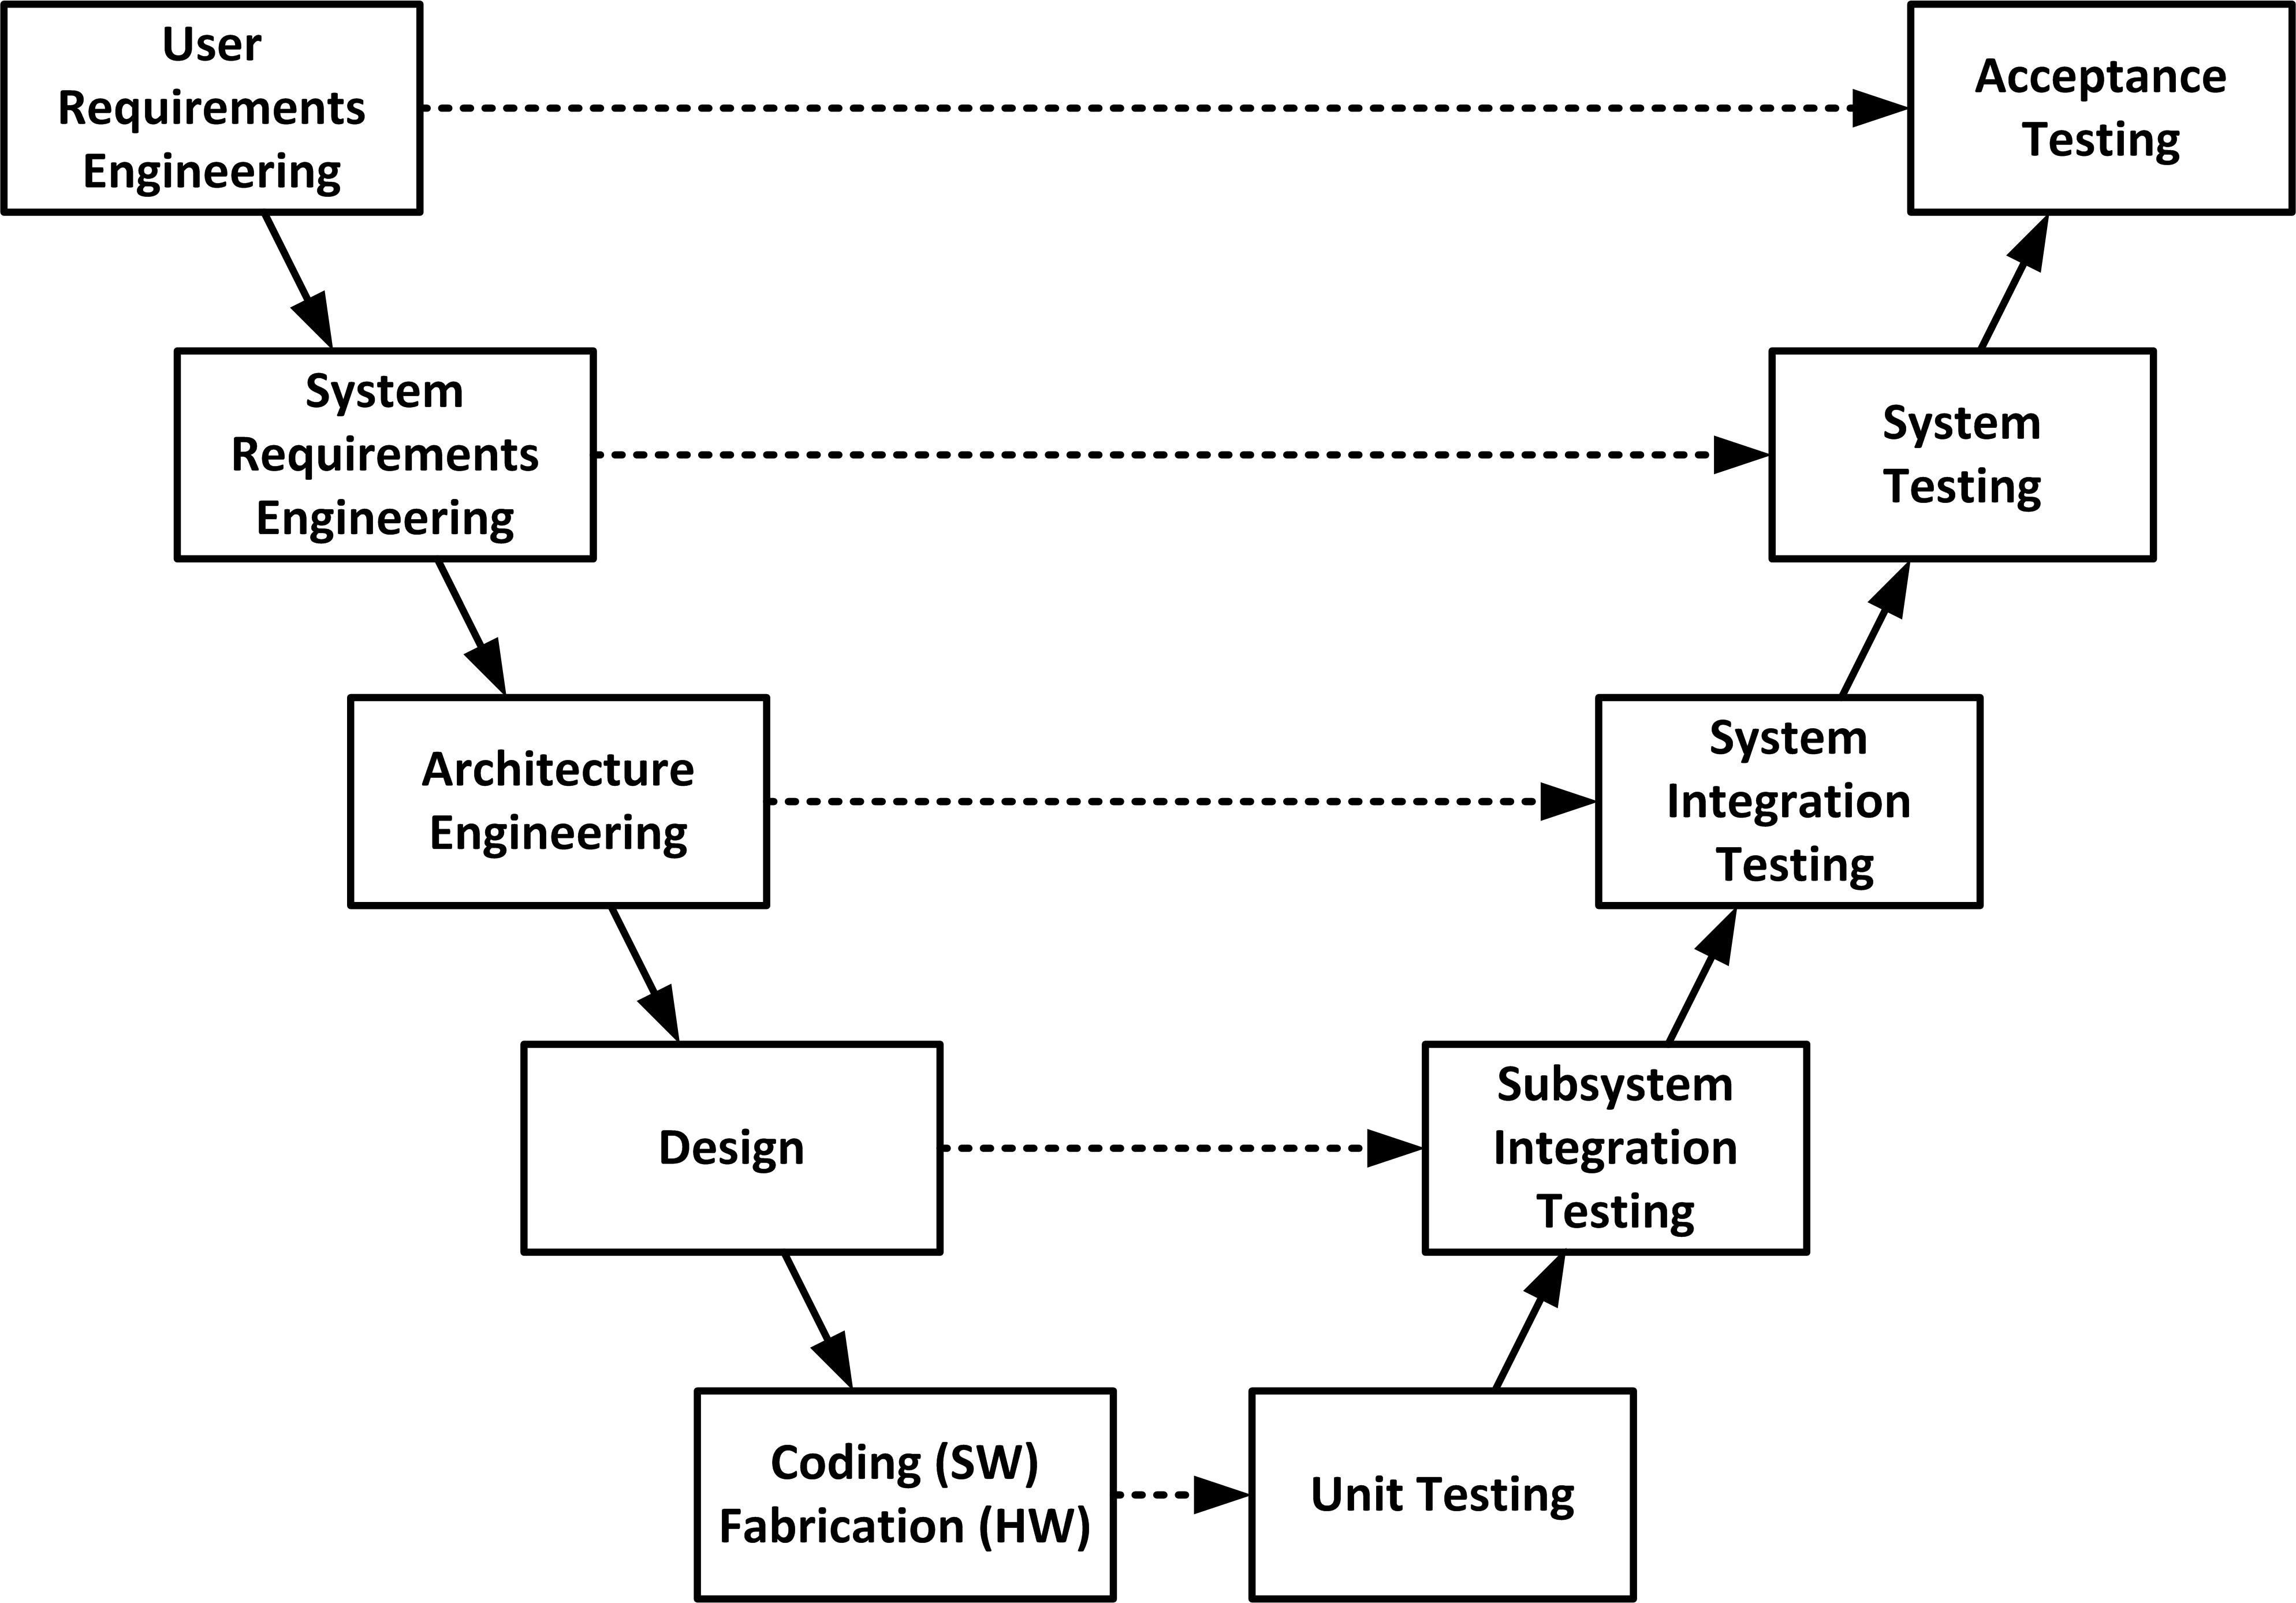
\includegraphics[scale=0.6]{res/images/v_model.jpg}
	\caption{Figura esplicativa del {modello a V}}
\end{figure}
\newline
Per definire lo stato dei test viene utilizzato un valore da 0 a 2:
\begin{itemize}
	\item \textbf{0:} il test non è stato implementato;
	\item \textbf{1:} il test è stato implementato, ma fallisce;
	\item \textbf{2:} il test è stato implementato e superato.
\end{itemize}
Vi sono quattro tipi di test:
\begin{itemize}
	\item accettazione;
	\item sistema;
	\item integrazione;
	\item unità.
\end{itemize}

\subsection{Test di Accettazione}
Verificano che il software nel suo complesso soddisfi i criteri di accettazione decisi con il cliente, verranno indicati nel seguente modo:\\
\begin{center}
	TA[Tipo]-[Codice]-[Importanza]\\
\end{center}
dove:
\begin{itemize}
    \item \textbf{Tipo:} indica il tipo dei requisiti\textsubscript{G} tra i seguenti tipi:
    \begin{itemize}
        \item \textbf{F} per i requisiti\textsubscript{G} funzionali;
        \item \textbf{V} per i requisiti\textsubscript{G} di vincolo;
        \item \textbf{Q} per i requisiti\textsubscript{G} di qualità;
        \item \textbf{P} per i requisiti\textsubscript{G} prestazionali.
    \end{itemize}
	\item \textbf{Codice:} rappresenta il codice identificativo crescente del componente da verificare.
	\item \textbf{Importanza:} indica l'importanza del requisito\textsubscript{G} che può essere:
		\begin{itemize}
			\item \textbf{O} per i requisiti\textsubscript{G} obbligatori;
			\item \textbf{D} per i requisiti\textsubscript{G} desiderabili;
			\item \textbf{F} per i requisiti\textsubscript{G} facoltativi.
		\end{itemize}
\end{itemize}

%tabella
	\begin{longtable}{ >{\centering}p{0.20\textwidth} >{}p{0.655\textwidth}
		>{\centering}p{0.15\textwidth}}% >{\centering}p{0.14\textwidth}}


	\caption{Riepilogo Test di Accettazione}\\
	\hline
	\rowcolorhead
	\headertitle{Requisito} & \headertitle{Descrizione} & \headertitle{Esito}
	\endfirsthead
	\caption[]{(continua)}\\
	\rowcolorhead
	\headertitle{Requisito} & \headertitle{Descrizione} & \headertitle{Esito}
	\endhead



	TAF-1-O & L'utente deve poter fare il login.\newline All'utente viene chiesto di: \begin{itemize}\item accedere alla pagina di login;\item inserire il proprio codice identificativo.\end{itemize} & 0\tabularnewline

	TAF-1.1-O & Se il codice non è corretto o non esiste nel sistema \newline il login fallisce.\newline Se il login dell'utente non va a buon fine deve venir mostrato un messaggio d'errore. & 0\tabularnewline

	TAF-2-O & L'amministratore deve poter registrare un nuovo account, di operatore o responsabile.\newline All'amministratore viene chiesto di: \begin{itemize}\item inserire nome lavoratore; \item inserire cognome lavoratore; \item inserire ruolo lavoratore (operatore o responsabile).\end{itemize} & 0\tabularnewline

	TAF-2.1-O & In caso di registrazione fallita (per lavoratore già esistente); allora deve venir mostrato un messaggio d'errore. & 0\tabularnewline

	TAF-3-O & L'amministratore può modificare un account già esistente di un lavoratore.\newline In particolare può: \begin{itemize}\item modificare campo nome; \item modificare campo cognome; \item modificare campo ruolo. \end{itemize} & 0\tabularnewline

	TAF-3.1-O & L'amministratore può eliminare un account già esistente. & 0\tabularnewline

	TAF-4-O & Il responsabile deve poter aggiungere una task\textsubscript{G} alla lista delle task\textsubscript{G}.\newline Al responsabile è richiesto di: \begin{itemize}\item autenticarsi con account con ruolo responsabile; \item selezionare il pulsante per aggiungere una nuova task\textsubscript{G}; \item inserire la priorità della task\textsubscript{G}; \item inserire il POI\textsubscript{A} a cui fa riferimento; \item confermare l'inserimento di nuova task\textsubscript{G}. \end{itemize} & 0\tabularnewline

	TAF-5-O & Il responsabile deve poter modificare la priorità di una task\textsubscript{G}.\newline Al responsabile è richiesto di: \begin{itemize}\item autenticarsi con account con ruolo responsabile; \item selezionare la task\textsubscript{G} da modificare; \item inserire la nuova priorità; \item confermare la modifica priorità della task\textsubscript{G}. \end{itemize} & 0\tabularnewline

	TAF-6-O & Il responsabile deve poter eliminare una task\textsubscript{G} dalla lista delle task\textsubscript{G}.\newline Al responsabile è richiesto di: \begin{itemize} \item autenticarsi con account con ruolo responsabile; \item selezionare la task\textsubscript{G} da eliminare; \item confermare l'eliminazione della task\textsubscript{G}. \end{itemize} & 0\tabularnewline

	TAF-7-O & Il sistema deve permettere all'utente di effettuare il logout dall'applicativo. & 0\tabularnewline

	TAF-7.1-O & Il sistema deve permettere all'operatore di effettuare il logout solo quando si trova in base.\newline All'utente è richiesto di: \begin{itemize} \item raggiungere la base; \item premere il pulsante logout nell'applicativo. \end{itemize} & 0\tabularnewline

	TAF-7.2-O & Il sistema deve permettere a responsabile e amministratore di effettuare il logout in qualsiasi momento.\newline Al responsabile/amministratore è richiesto di: \begin{itemize} \item premere il pulsante logout nell'applicativo. \end{itemize} & 0\tabularnewline

	TAF-8-O & Il sistema deve permettere a responsabili e amministratore di visualizzare la mappa, e in particolare visualizzare i POI\textsubscript{A}, aree non transitabili, muletti in real-time e le zone di percorrenza\textsubscript{G}.\newline All'utente è richiesto:\begin{itemize} \item autenticarsi come responsabile o amministratore; \item selezionare il pulsante per la visualizzazione della mappa; \item visualizzare i vari elementi della mappa (POI\textsubscript{A}, zona di percorrenza\textsubscript{G}, aree non transitabili e muletti in real-time). \end{itemize} & 0\tabularnewline

	TAF-8.1-F & Il sistema deve permettere agli utenti la visualizzazione delle persone in real-time sulla mappa & 0\tabularnewline

	TAF-9-O & Il sistema deve permettere all'amministratore la visualizzazione di una notifica in caso della segnalazione da parte di un utente di un evento eccezionale. & 0\tabularnewline

	TAF-10-O & Il sistema deve permettere all'amministratore di modificare la mappa, in particolare modificare planimetria\textsubscript{G} e percorrenza\textsubscript{G}.\newline All'utente è richiesto: \begin{itemize} \item autenticarsi come amministratore; \item selezionare il pulsante per la gestione mappa; \item selezionare il pulsante relativo alla modifica della mappa da effettuare.\end{itemize} & 0\tabularnewline

	TAF-10.1-O & Il sistema deve permettere all'amministratore di gestire i POI\textsubscript{A} nella mappa, in particolare modificarne la posizione di uno già esistente.\newline All'amministratore è richiesto: \begin{itemize}\item autenticarsi come amministratore; \item selezionare il pulsante per la gestione mappa; \item selezionare il pulsante per la gestione dei POI\textsubscript{A}; \item selezionare il pulsante per la modifica della posizione di un POI\textsubscript{A}; \item selezionare il POI\textsubscript{A} interessato e aggiornarne la posizione.\end{itemize} & 0\tabularnewline

	TAF-10.2-O & Il sistema deve permettere all'amministratore di eliminare un POI\textsubscript{A} già esistente.\newline All'amministratore è richiesto: \begin{itemize}\item autenticarsi come amministratore; \item selezionare il pulsante per la gestione mappa; \item selezionare il pulsante per la gestione dei POI\textsubscript{A}; \item selezionare il POI\textsubscript{A} da eliminare; \item selezionare il pulsante di eliminazione del POI\textsubscript{A}.\end{itemize} & 0\tabularnewline

	TAF-10.3-O & Il sistema deve permettere all'amministratore di creare un nuovo POI\textsubscript{A}.\newline All'amministratore è richiesto: \begin{itemize}\item autenticarsi come amministratore; \item selezionare il pulsante per la gestione mappa; \item inserire codice identificativo, posizione nella mappa, tipo di POI\textsubscript{A} (carico, scarico, base) del nuovo POI\textsubscript{A}; \item selezionare il pulsante di conferma dell'aggiunta del POI\textsubscript{A}.\end{itemize} & 0\tabularnewline

	TAF-11-O & L'operatore deve poter accedere alla sua user interface. All'utente è richiesto di: \begin{itemize} \item autenticarsi come operatore; \item selezionare il pulsante per accedere alla user interface.\end{itemize} & 0\tabularnewline

	TAF-11.1-O & L'operatore deve poter vedere sotto alla mappa una lista ordinata delle task\textsubscript{G} rimanenti da eseguire dall'operatore.\newline All'utente è richiesto di: \begin{itemize} \item autenticarsi come operatore; \item selezionare il pulsante per accedere alla user interface; \item nella user interface raggiunta, sotto la mappa deve apparire una lista ordinata contenente le task\textsubscript{G} rimanenti da soddisfare.\end{itemize} & 0\tabularnewline

	TAF-11.2-O & L'operatore deve poter vedere nella mappa il prossimo task\textsubscript{G} da soddisfare(POI\textsubscript{A} da raggiungere) (evidenziato con colore diverso).\newline All'utente è richiesto: \begin{itemize} \item autenticarsi come operatore; \item selezionare il pulsante per accedere alla user interface; \item nella user interface raggiunta, nella mappa deve mostrare il prossimo task\textsubscript{G} da raggiungere.\end{itemize} & 0\tabularnewline

	TAF-11.3-O & L'operatore deve poter segnalare la conclusione dell'incarico attraverso la user interface.\newline All'utente è richiesto: \begin{itemize} \item autenticarsi come operatore; \item selezionare il pulsante per accedere alla user interface; \item nella user interface raggiunta, l'operatore deve cliccare sul POI\textsubscript{A} evidenziato (raggiunto) nella mappa e confermare l'avvenuto scarico.\end{itemize} & 0\tabularnewline

	TAF-11.4-O & L'operatore deve poter vedere direzione e spostamento del muletto a cui è a bordo, in caso sia attiva la guida automatica; in particolare il sistema deve attivare le icone di frecce direzionali, start e stop.  & 0\tabularnewline

	TAF-11.5-O & L'operatore deve poter passare da guida manuale a guida automatica attraverso la user interface.\newline All'utente è richiesto: \begin{itemize} \item autenticarsi come operatore; \item accedere alla user interface, attraverso l'apposito pulsante; \item selezionare il pulsante per cambiare tipo di guida (manuale, automatica). \end{itemize} & 0\tabularnewline

	TAF-11.6-O & L'operatore deve poter segnalare un evento eccezionale al server attraverso la user interface.\newline All'utente è richiesto: \begin{itemize} \item autenticarsi come operatore; \item accedere alla user interface, attraverso l'apposito pulsante; \item segnalare un evento eccezionale, attraverso l'apposito pulsante.\end{itemize} & 0\tabularnewline

	TAF-11.7-O & L'operatore deve poter impostare la guida automatica verso la base, dopo aver finito tutte le task\textsubscript{G}, attraverso l'apposito pulsante nella user interface.\newline All'utente è richiesto: \begin{itemize} \item autenticarsi come operatore; \item accedere alla user interface, attraverso l'apposito pulsante; \item dopo aver finito tutte le task\textsubscript{G}, appare un pulsante per ritornare alla base con guida automatica.\end{itemize} & 0\tabularnewline

	TAF-11.8-O & La user interface che rappresenta una singola unità, deve prevedere pulsanti per 4 frecce direzionali, start e stop per gli spostamenti manuali. & 0\tabularnewline

	TAF-12-D & Il pannello permette di visualizzare l'indicatore di velocità attuale. & 0\tabularnewline

	TAF-13-O & Il sistema centrale deve pilotare e coordinare tutte le unità per evitare ingorghi e incidenti. & 0\tabularnewline

	TAF-13.1-F & Il sistema fornisce il percorso migliore alle unità tramite algoritmi di ricerca operativa. & 0\tabularnewline

	TAF-14-O & Il sistema deve permettere a amministratore e responsabili di visualizzare la lista di tutti i POI\textsubscript{A} presenti nella mappa. & 0\tabularnewline

	TAF-15-O & Il responsabile deve poter vedere la lista completa delle task\textsubscript{G}.\newline All'utente è richiesto:\begin{itemize} \item autenticarsi come responsabile; \item selezionare il pulsante per visualizzare la lista completa delle task\textsubscript{G}. \end{itemize} & 0\tabularnewline

	TAF-16-O & L'amministratore deve poter accedere a un'interfaccia per aggiungere o rimuovere un'unità.\newline All'utente è richiesto: \begin{itemize} \item autenticarsi come amministratore; \item accedere all'interfaccia per gestire le unità, con l'apposito pulsante.\end{itemize} & 0\tabularnewline

	TAF-16.1-O & L'amministratore deve poter aggiungere un'unità. \newline All'utente è richiesto: \begin{itemize} \item autenticarsi come amministratore; \item accedere all'interfaccia per gestire le unità, con l'apposito pulsante; \item selezionare il pulsante per aggiungere una nuova unità; \item inserire il codice identificativo dell'unità; \item confermare l'aggiunta della nuova unità.\end{itemize} & 0\tabularnewline

	TAF-16.2-O & L'amministratore deve poter rimuovere un'unità. \newline All'utente è richiesto: \begin{itemize} \item autenticarsi come amministratore; \item accedere all'interfaccia per gestire le unità, con l'apposito pulsante; \item selezionare il pulsante per rimuovere un'unità; \item selezionare l'unità da rimuovere; \item confermare la rimozione dell'unità.\end{itemize} & 0\tabularnewline



\end{longtable}
%fine tabella

\subsection{Test di Sistema}
I Test di Sistema verificano la conformità dell'intero sistema con i requisiti\textsubscript{G} specificati.\\I Test di Sistema verranno sviluppati quando verrà raggiunta la fase\textsubscript{G} appropriata, secondo il modello a V\textsubscript{G}.

\subsection{Test di Integrazione}
I Test di Integrazione verificano l'integrazione di più componenti software o hardware.\\I Test di Integrazione verranno sviluppati quando verrà raggiunta la fase\textsubscript{G} appropriata, secondo il modello a V\textsubscript{G}.

\subsection{Test di Unità}
I Test di Unità verificano le parti atomiche del software (per esempio funzioni o procedure). Vengono utilizzati per assicurarsi che la logica interna del codice sia rispettata.\\I Test di Unità verranno sviluppati quando verrà raggiunta la fase\textsubscript{G} appropriata, secondo il modello a V\textsubscript{G}.
